% !TeX encoding = utf8
% !TeX spellcheck = de-DE


\chapter{Projekt}

%\makeatletter
%\renewcommand{\caption}{\@makecaption[2]{\centering   \vskip\abovecaptionskip
%\bfseries}}
%\makeatother


\section{Fokus des Programms}

Das Programm Antz legt einen Schwerpunkt auf die visuelle Veranschaulichung des
Ameisenkoloniealgorithmus und das Spiel mit dem Einfluss verschiedener Parameter
auf die Lösungsfindung. Funktionell geht es primär um die Lösung des Problems
des kürzesten Weges. Allerdings wird mit diesem Programm kein spezifisches
Problem wie beispielsweise das TSP effizient gelöst, sondern unterschiedliche
Probleme sollen sich rasch lösen lassen. Die zugrunde liegende Berechnung
erfolgt nicht besonders effizient, da dieser Aspekt nicht im Fokus der
Entwicklung stand.


% (Animation, Multi-Purpose [kein spezifisches Problem effizient gelöst, sondern
%mehrere Probleme rasch lösen können]; nicht effiziente Berechnung)



\section{Vorgehen}

Zur Projektverwaltung und Publikation wurde ein Repository auf
GitHub\footnote{\url{https://github.com/jajadinimueter/antz}} verwendet. In
einem Ordner «docs» sind die wesentlich Dokumente aus unserer
Projektdokumentation abgelegt. Für die Planung der Meilensteine und Iterationen
wurde ein eigenes Konto unter
TargetProcess\footnote{\url{http://jajadinimueter.tpondemand.com}} verwendet.

Für die gemeinsame Arbeit an der Dokumentation eröffneten wir zuerst einen
Account bei einem Online LaTeX Editor\footnote{\url{http://www.sharelatex.com}}.
Später entdeckten wir eine praktische LaTeX-Vorlage von Matthias
Pospiech\footnote{\url{http://www.matthiaspospiech.de/latex/vorlagen/allgemein}},
mit dem fortan die Dokumenation verfasst wurde. Da für die Verwendung dieser
Vorlage die Möglichkeiten von sharelatex.com zu wenig ausgeprägt waren und das
Kompilieren zu langsam vor sich ging, wurde entschieden, die LaTeX-Dokumentation
ebenso über Git zu pflegen.

Die regelmässige Kommunikation unter beiden Projektpartnern erfolgte entweder in
direktem mündlichen Austausch oder per E-Mail oder per Chat. Um das Projekt
besser voranzubringen, trafen wir uns zudem mehrere Male für die direkte Arbeit
am Programm oder an der Dokumentation.



\section{Projektplanung}

Bei der Planung für dieses Softwareprojekt waren drei Meilensteine
anzusetzen.\footnote{Vgl. auch die Screenshots aus dem verwenden
Projektplanungstool in Anhang \ref{sec:planungstool}.} Für die einzelnen
Meilensteine wurden vier, drei und fünf Wochen angesetzt. Erwartungsgemäss
dauerte der letzte Meilenstein etwas länger, wofür eine entsprechende Reserve
von zwei Wochen eingeplant war.

Zur effizienten Planung der drei Zwischenabgaben\footnote{Die drei Abgabereporte
finden sich in Anhang A.} war das folgende Planungsdreieck zweckdienlich.
Insbesondere auch für die Priorisierung noch ausstehender User Stories innerhalb
und zwischen den drei Meilensteinen. \\

\begin{figure}[h]
  \centering
	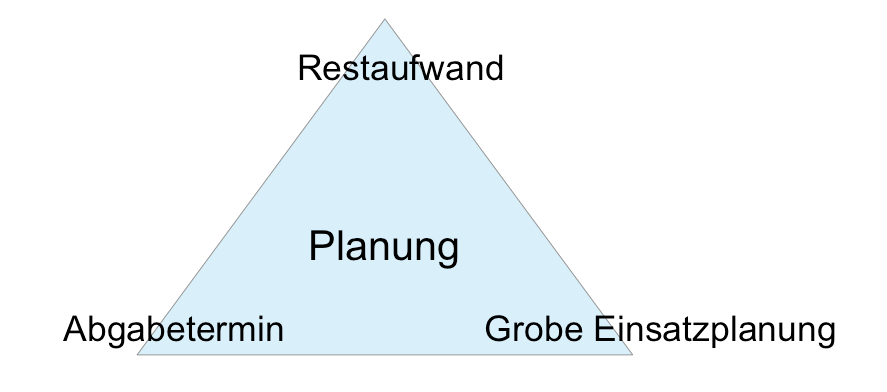
\includegraphics [width=0.65\textwidth]{images/Planungsdreieck.png}
	\caption{Planungsdreieck (Quelle: Einführende Präsentation von Syrus Mozafar)}
\end{figure}

\noindent
Der offizielle Projektplan gab folgende äussere Rahmenbedingungen vor:

%\FloatBarrier
\begin{table}[H]
\small\sffamily\renewcommand{\arraystretch}{1.5}
\begin{tabular}{| p{2.5cm} | l |}
  \hline
  \bfseries{Datum} & \bfseries{Ziel}  \\
  \hline
  26.02.2014 & Wahl des Themas, Gruppenbildung \\ 
  \hline
  Anschliessend & Besprechung mit Fachdozent \\
  \hline
  12.03.2014 & Erste Besprechung mit Syrus Mozafar \\
  \hline
  24.03.2014 & Erste Abgabe des Projektzwischenstandes \\
  \hline
  14.04.2014 & Zweite Abgabe des Projektzwischenstandes \\
  \hline
  05.05.2014 & Dritte Abgabe des Projektzwischenstandes \\
  \hline
  30.05.2014 & Abgabe des Projektes \\
  \hline
  04./11.06.2014 & Präsentation des Projektes \\
  \hline
\end{tabular}
\captionsetup{type=table} % unnötig?
\caption{Offizielle Fixpunkte der Projektplanung}
\end{table}

\newpage

\subsection{Meilenstein 1: Arthur}

\vbox{
Im ersten Meilenstein Arthur bestand das Ziel darin, das Programm mit einigen
grundlegenden Funktionen lauffähig zu erstellen. Hier die entsprechende
Beschreibung aus unserem Planungstool:

\begin{itemize}[noitemsep]
\item A prototype of moving ants, pheromones and food piles MUST be created.
\item There will be some UI controls like sliders to adjust some values.
\item The exact algorithm MUST NOT be implemented. But ants want to find food
and return to the hive when found. \\\\
\end{itemize}
}

% \renewcommand{\arraystretch}{2}	% vor einer Tabelle

\begin{table}[H]
\small\sffamily\renewcommand{\arraystretch}{1.5}
\begin{tabular}{| p{12cm} | c | c |}
  \hline
  \bfseries{User Story} & \bfseries{Sch.} & \bfseries{Eff.}  \\
  \hline
  As beginner in Python I have to work through a tutorial. & 10\,pt & 12\,pt \\
  \hline
  As a developer I want to make sure that UI controls can be placed on the
surface. & 1\,pt &1\,pt \\
  \hline
  As a windows user I want to be provided with an EXE file. & 1\,pt &4\,pt \\
  \hline
  As a user I want to see a surface with moving sprites on it. & 0.5\,pt & 6\,pt
\\
  \hline
  As a developer I want to see ants choosing randomly between n different
directions. & 5\,pt & 5\,pt \\
  \hline
  As a user I want to see at least 10000 ant-sprites on the surface without
significant lag. & 0.5\,pt & 0.5\,pt \\
  \hline
  As a user I want to see ants and food piles on the surface. & 4\,pt & 4\,pt \\
  \hline
  As a user I want to see ants disassociate pheromones. & 3\,pt & 4\,pt \\
  \hline
  As a user I want to see all ants spawning at a certain location. The nest. &
2\,pt & 2\,pt \\
  \hline
  As a user I want a visual feedback of pheromone evaporation. & 1\,pt & 1\,pt
\\
  \hline
  As a user I want to see ants react on pheromones. Ants have to go in the
direction of pheromones. & 1\,pt & 1\,pt \\
  \hline
  As a user I want to draw food piles on the surface. & 10\,pt & 10\,pt \\
  \hline
\end{tabular}
\captionsetup{type=table} % unnötig?
\caption{User Stories des ersten Meilensteines}
\end{table}

\subsubsection*{Fazit}

Diese Iteration war sehr erfolgreich, da wir bereits eine lauffähige Lösung produzieren
konnten. Auch die eingeplanten Stunden konnten wir relativ gut einhalten. Nur den
Aufwand, um die Simulation soweit mit pyGame zu verknüpfen, dass sich bewegende Sprites
angezeigt werden, haben wir unterschätzt.

\subsection{Meilenstein 2: Cobannus}

\vbox{
Für den zweiten Meilenstein Cobannus galt es folgendes Ziel zu erreichen:

\begin{itemize}[noitemsep]
\item This release includes the fully working solution including finding the
shortest path through a set of points.
\end{itemize}
}

\begin{table}[H]
\small\sffamily\renewcommand{\arraystretch}{1.5}
\begin{tabular}{| p{12cm} | c | c |}
  \hline
  \bfseries{User Story} & \bfseries{Sch.} & \bfseries{Eff.}  \\
  \hline
  As a user I want to see ants go directly to the nest after reaching the food
pile. & 1\,pt & 1\,pt \\
  \hline
  As a user I want to influence the pheromone evaporation. & 1\,pt & 0.5\,pt \\
  \hline
  As a user I want to see ants searching the shortest path through n points. &
4\,pt & 6\,pt \\
  \hline
  As a user I want to be able to define the number of ants available. & 2\,pt &
0.5\,pt \\
  \hline
  As a user I want to be able to place obstacles in the way of the ants. & 5\,pt
& 3\,pt \\
  \hline
  As a user I want to see the ants dynamically adjust their path when obstacles
are added. & 1\,pt & 2\,pt \\
  \hline
  As a user I want to have a mode which shows only the shortest path through the
points. & 1\,pt & 1\,pt \\
  \hline
\end{tabular}
\caption{User Stories des zweiten Meilensteines}
\end{table}

\subsubsection*{Fazit}

Auch eine sehr erfolgreiche Iteration. Alle Stories konnten abgearbeitet werden und die
Abweichungen von der Schätzung hielten sich im Rahmen. In dieser Iteration
implementierten wir den Algorithmus, der zu einem kürzesten Pfad führen sollte. Leider
war diese Lösung sehr defizitär. Was diese Iteration im Nachhinein etwas schlechter
aussehen lässt.

\subsection{Meilenstein 3: Tarvos}

Im dritten Meilenstein Tarvos waren folgende Ziele zu erreichen:

\begin{itemize}[noitemsep]
\item This release includes additional features like food piles with different
amount of glucose, food pile disintegration and so on.
\item Furthermore, additional UI controls may be added to configure all aspects
of the algorithm
\end{itemize}

\begin{table}[H]
\small\sffamily\renewcommand{\arraystretch}{1.5}
\begin{tabular}{| p{12cm} | c | c |}
  \hline
  \bfseries{User Story} & \bfseries{Sch.} & \bfseries{Eff.}  \\
  \hline
  Documentation and presentation. & 10\,pt & 15\,pt \\
  \hline
  As a user I want to define the glucose content of different food piles. &
  1\,pt & - \\
  \hline
  As a user I expect the ant collecting the food with most glucose content first. & 2\,pt & - \\
  \hline
  As a user I expect the ants collecting the food. Means the amount of food decreases over time. & 2\,pt & - \\
  \hline
  Documentation and Presentation (II). & 10\,pt & 10\,pt \\
  \hline
\end{tabular}
\captionbelow{User Stories des dritten Meilensteines}
\end{table}

\subsubsection*{Fazit}

Der Meilenstein ``Tarvos'' konnte nicht wie geplant durchgeführt werden, da 
bereits viel Zeit in Refactoring-Arbeiten und Anpassungen des Algorithmus 
investiert wurde. Zentrale Eigenschaften des Algorithmus wurden erst in dieser
Iteration verstanden und mussten noch entsprechend angepasst werden. Dazu 
gehören die Normierung aller Werte auf das Interval $[0,1]$ und die Bedeutung
der Exponenten.

\section{Technologien}


